\section{Versuchsbeschreibung}
\subsection{Versuchsaufbau}
Der Versuchsaufbau besteht aus einer Lampe die hinter einer verstellbaren 
Spaltblende montiert wird. Vor die Spaltblende wird eine Halterung für 
Farbfilter und eine Sammellinse montiert. Als letztes Bauteil auf der 
Optischen Bank wird ein Podest benötigt auf welches während der 
Versuchsdurchführung Prismen gestellt werden können. Vor das Podest wird 
nun ein Schirm mit einer montierten Skala aufgebaut. Das Podest hat eine 
Entfernung von 38,5 cm zum Schirm.
\begin{figure}[!htb]
\centering
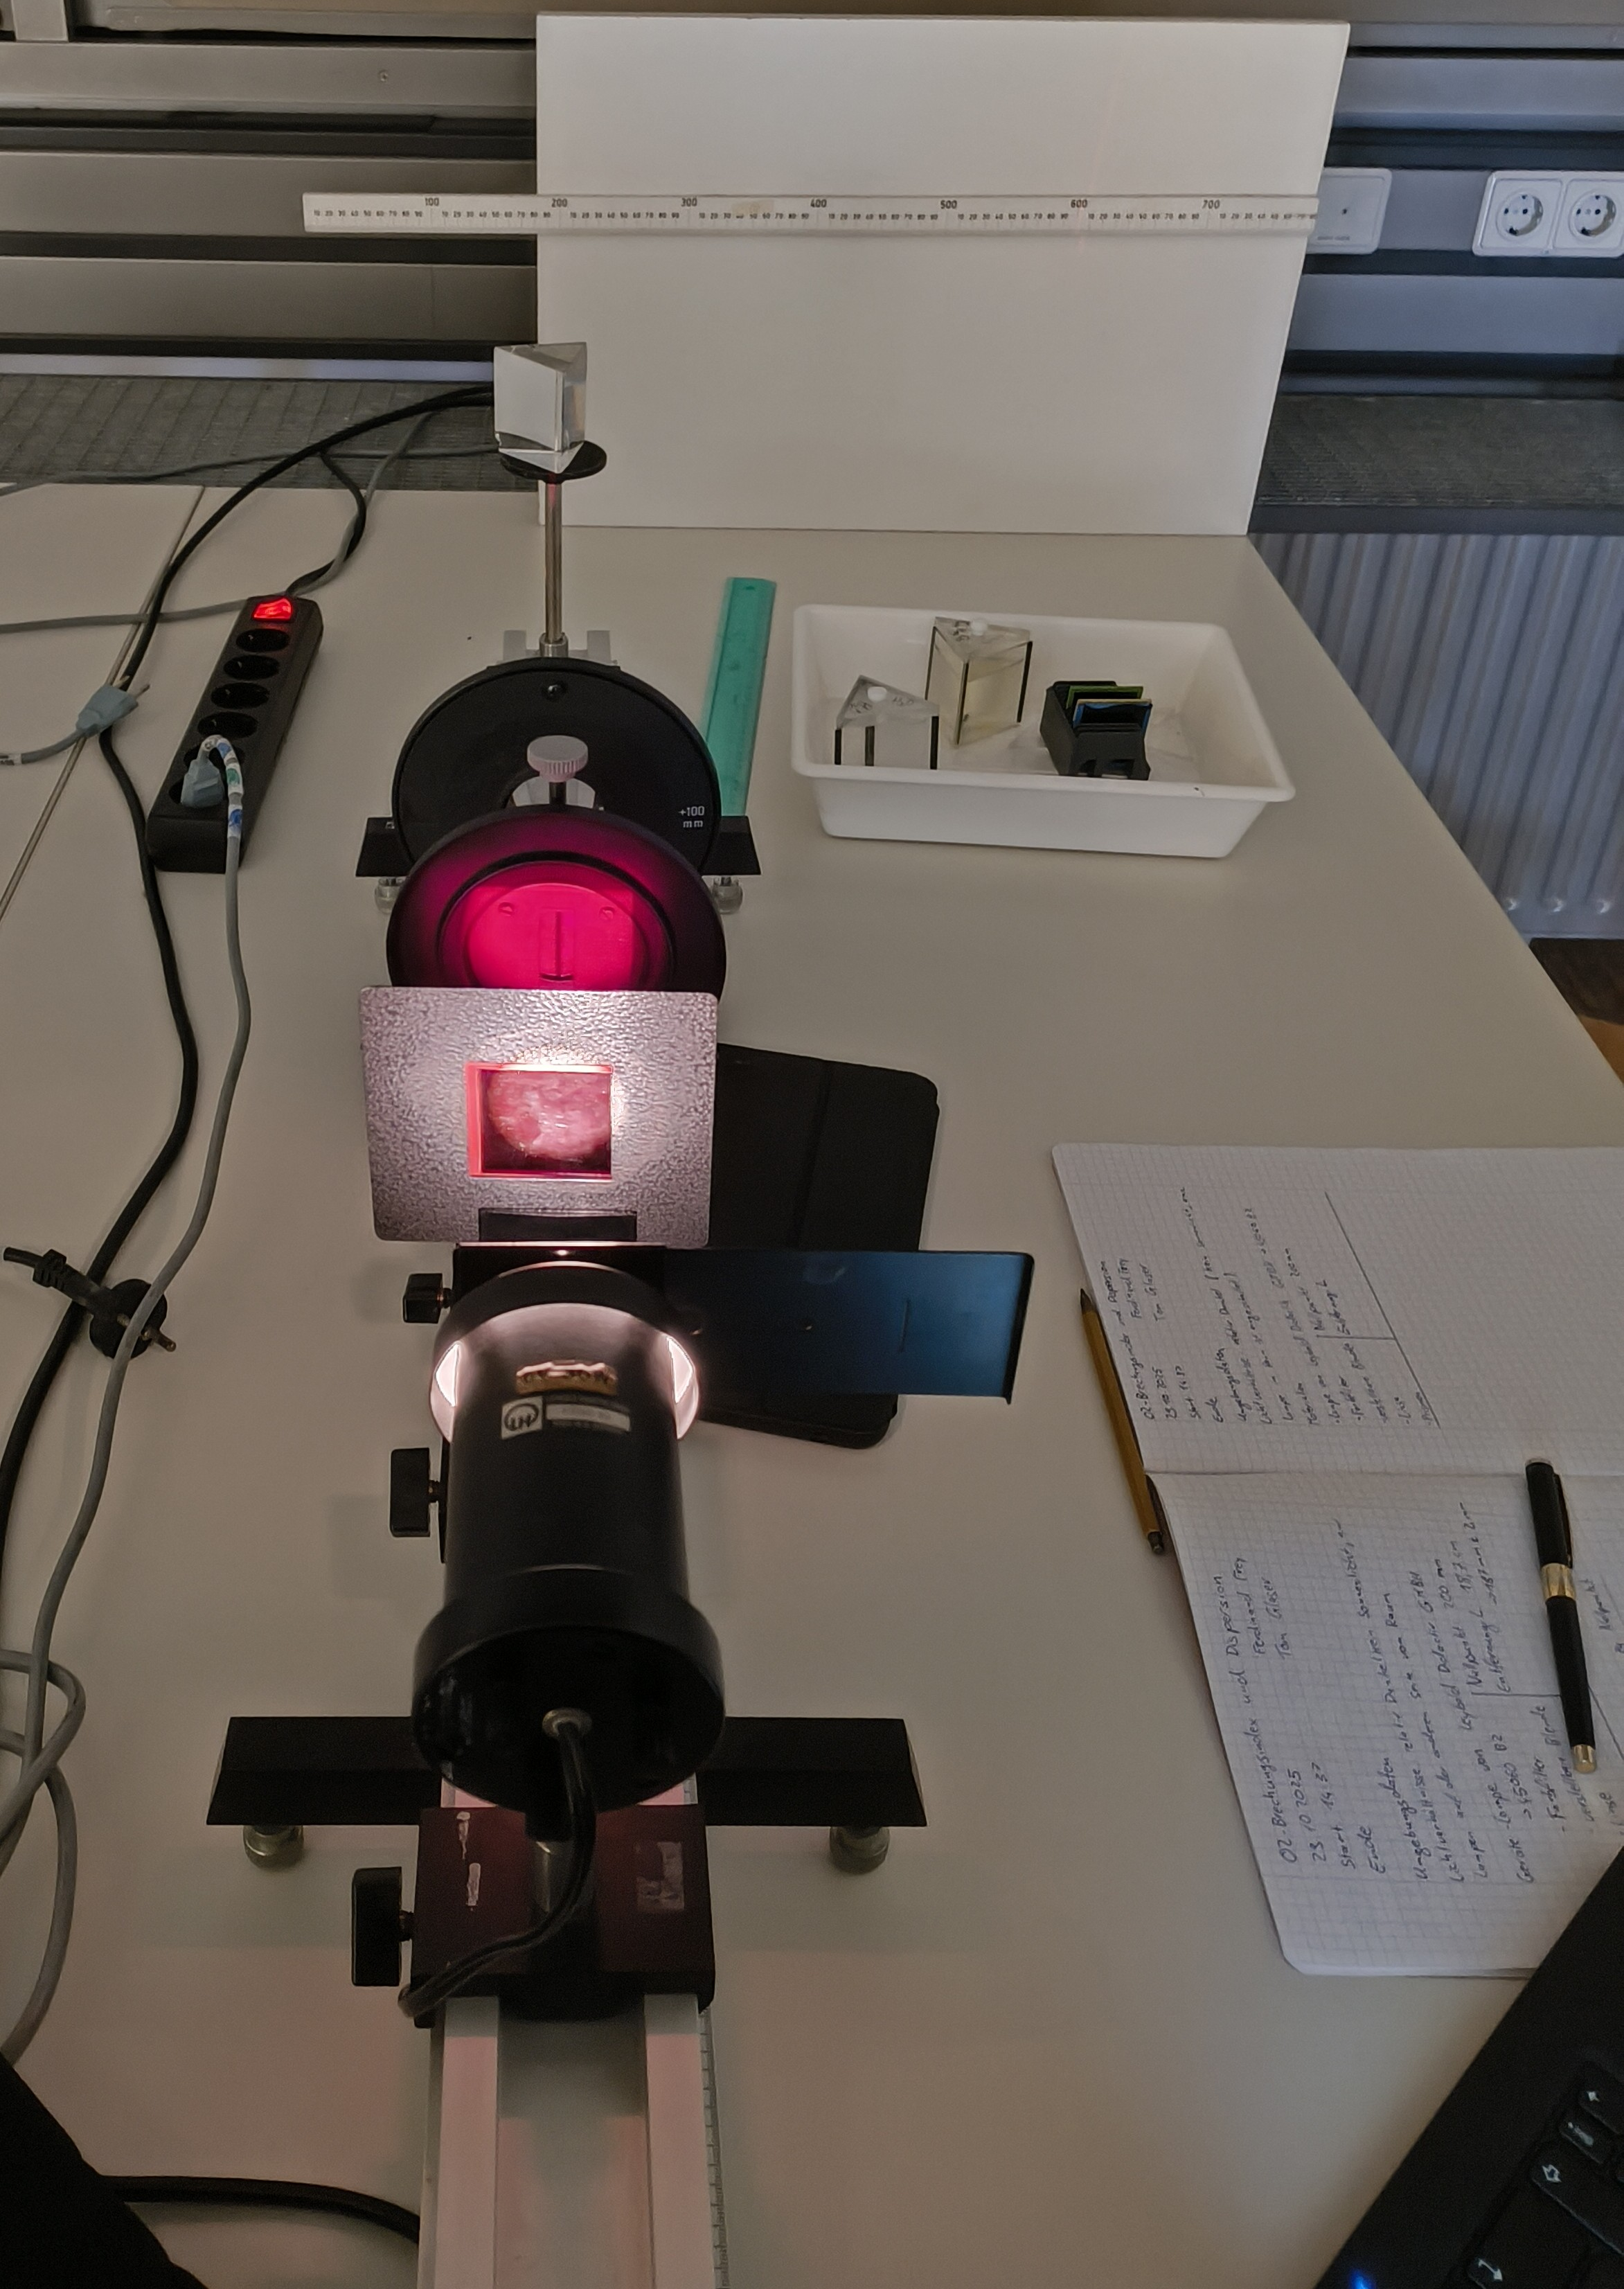
\includegraphics[scale=0.08]{Bilder/Richtiger Aufbau.jpg}
\caption{Ein Bild vom Versuchsaufbau, von vorne nach hinten. Lampe, Spaltblende, Farbfilterhalterung, Sammellinse, Podest und Schirm.  }
\end{figure}

%\begin{wrapfigure}{r}{0.4\textwidth} % r=rechts, l=links, 0.4=Breite 
%        \centering
%        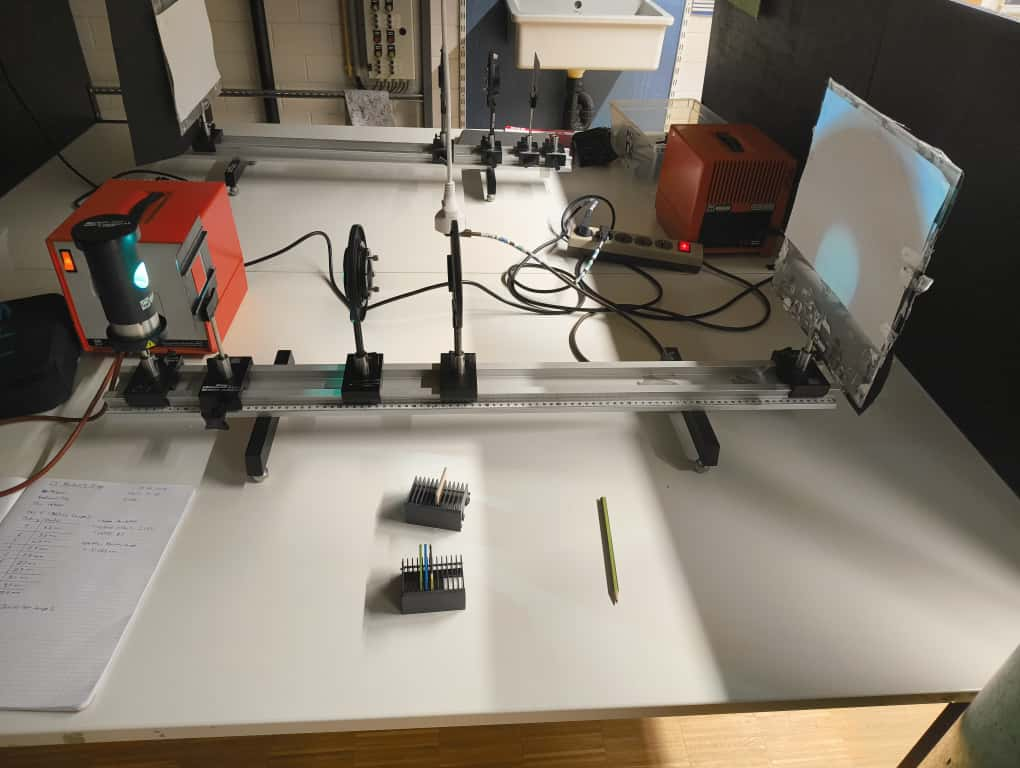
\includegraphics[width=0.9\linewidth]{Bilder/Versuchsaufbau O3.jpeg}
%        \caption{Versuchsaufbau}
%       \label{fig:SpASkizze}
%\end{wrapfigure}


\subsection{Versuchsdurchführung}
